\chapter{Appendices}

\renewcommand*{\chaptermarkformat}{}
\section{Plots of Functions of a Complex Variable} \label{sec:f(z)}
\chaptermark{Appendix 1. Plots of Functions of a Complex Variable}

\begin{figure}
 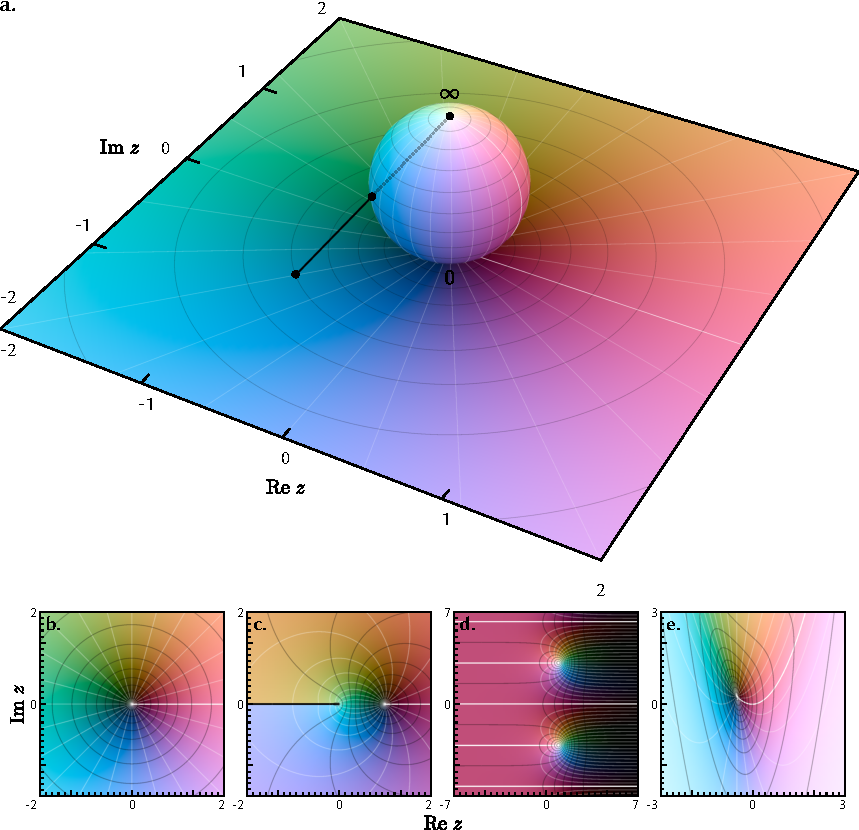
\includegraphics{figs/app/Riemann.pdf}
 \caption[Riemann sphere and complex plots]{\small \label{fig:riemann}
 \textbf{Riemann sphere and complex plots.}\small\\
 \subA. projection of the Riemann sphere onto the complex plane, each point on
 the sphere is assigned a unique colour, which maps to the extended complex
 plane.\\
 \subB, \subC, \subD, \subE. show complex plots of the following functions:
 \\
 \subB. Identity function, $f(z) = z$, zeros show in black as sources of contour
 lines.
 \\
 \subC. Logarithm, $f(z) = \log z$, note the branch cut along the negative real
 axis.
 \\
 \subD. Fermi Function, $f(z) = (1+\exp(z-1))^{-1}$, poles here are shown in
 white and are sinks of contour lines.
 \\
 \subE. Non-analytic function, $f(x+iy)=1+2 x + i y - i x^2$. Non-analytic
 functions are not conformal maps in the complex plane, producing contours that
 do not intersect at right angles.
 }
\end{figure}

In this thesis, it has occasionally been necessary to plot functions of a complex
variable.
These functions are often difficult to visualise since they map one pair of
real variables to another $f: x + i y \→ u + i v$, requiring four dimensions
in total for the domain and the range.

Here functions of a complex variable are plotted as \twod colour plots, where
the range of the function is mapped to a colour that is plotted over the domain.

Colours are assigned such that every point on the extended complex plane
$\hat{\mathbb{C}}$ (Complex numbers and the point at infinity) is uniquely
coloured.
Here $\hat{\mathbb{C}}$ is mapped to the Riemann sphere,
defined as the points labelled with polar angles $(\θ,\φ)$ on a sphere of radius
$\nicefrac{1}{2}$ that touches the complex plane at $0$ at its base, as depicted
in \fig{riemann}.
Points on the complex plane are mapped to the sphere by a construction where a
line is drawn from the top of the sphere to a point on the plane; the point is
mapped to the intersection of that line and the sphere.
This is expressed more concisely as $(\θ(r), \φ) = r e^{i\φ} \→ (2
\arccot r,\φ)$.

The sphere is coloured in a CIE L*a*b* colour space, with the top point being
white, the bottom black, with the saturation maximal around the equator
(representing unit complex numbers).
The phase maps to the hue of the colour, with red being real positive
numbers.
The \emph{lab} colour space has the advantage that it is “perceptually uniform”,
which is to say that colours that vary only by hue, look the same brightness and
saturation to a human eye.
This will avoid spurious bright bands that appear in an sRGB colour space.

In the plots, contours are drawn for constant amplitude in black, and constant
phase in white.
Analytic functions are conformal maps - they preserve angles, therefore plots of
analytic functions will have their contours intersect at right-angles (except at
singular points and zeros, and points of zero derivative).
In such a depiction, roots and poles are sources and sinks of contours of
constant phase, and are circled by contours of constant amplitude, with roots
being a black point, and poles being a white point.
Branch points are drawn in this plot as thicker black lines.
This is depicted in examples in \fig{riemann} in addition to a function that is
not analytic hence not a conformal map.

\section{Branches of the Polarisability Function} \label{sec:branchcuts}
\chaptermark{Appendix 2. Branches of the Polarisability Function}

The dimensionless polarisability of zero temperature doped graphene, given in
\eq{analPolar}, is a multi-valued function of a complex variable.
The function, as given, has branch cuts, and a straight evaluation will return
the principal branch.
In the analysis of \sec{cfpd}, it can be required that the function needs to be
analytically continued over a branch cut.

Here the functions $\Πtil_1$, $\Πtil'$, and $\Πtil_0$ are presented as functions
of a complex $\ωtil$ for constant $\qtil$, with the additional dependence of a
branch parameter $\ξ$, which is a list of integers.

The original functions are,
\begin{subequations}\subeq
\begin{align}
\Πtil_1(\qtil, \ωtil) &=
-4 + \qtilAbs^2 \frac{G^{+}(\frac{2+\ωtil}{\qtilAbs}) +
G^{-}(\frac{2-\ωtil}{\qtilAbs})}{2
\sqrt{\qtilAbs^2 - \ωtil^2}}
\\
\Πtil'(\έtil; \qtil, \ωtil) &=
-4 + 2 \frac{
\Gp \left( \frac{\ωtil + 2 \έtil}{\qtilAbs} \right) +
\Gp \left( \frac{\ωtil - 2 \έtil}{\qtilAbs} \right)
}{
\Gp \left( \frac{\ωtil}{\qtilAbs} \right)
}
\\
\Πtil_0(\qtil, \ωtil) &= -\frac{\qtilAbs}{2} \frac{\π}{\Gp \left(
\frac{\ωtil}{\qtilAbs} \right) }
\;,
\end{align}
\end{subequations}
with,
\begin{subequations}\subeq
\begin{align}
G^{\pm}(z) &= z \sqrt{1-z^2} \pm \i \arccosh(z)
\\
\Gp(z) &= \sqrt{1 - z^2}
\;.
\end{align}
\end{subequations}
The branch cuts originate from square-root and logarithmic (arccosh) branch
point singularities.

Redefining the auxiliary functions as,
\begin{subequations}\subeq
\begin{align}
\Gp_{m,n}(z) &=
e^{i \π/2 (n + m)} \sqrt{e^{-i \π (n + 1/2)} (z - 1)} \sqrt{
  e^{-i \π (m + 1/2)} (z + 1)}
\\
G_{m,n,p}(z) &=
z \Gp_{m, n}(z) + i \log\left(e^{-i \π (p + 1/2)} (z + i \Gp_{m, n}(z))\right)
- \π p
\;.
\end{align}
\end{subequations}
sets each branch cut to be angled vertically downwards along the negative
imaginary axis.
$m$ controls the branch cut at $z=-1$ and $n$ at $z=+1$.
By incrementing or decrementing this value, the branch is rotated
counter-clockwise 180°.
$p$ controls the branch of the logarithm, is set such that it's branch cut is
not exposed, but is rather hidden in the other leaf of the square root.

The polarisability functions can then be set such that all the branch cuts point
downwards in $\ωtil$.
In the general case, this is controlled by eight integers:
\begin{subequations}\subeq
\begin{align}
\Πtil_1(\qtil, \ωtil; \ξ) &=
-4 + \qtilAbs \frac{
G_{\ξ_1, \ξ_2, \ξ_3}\left( \frac{\ωtil + 2}{\qtilAbs} \right) -
G_{\ξ_6, \ξ_7, \ξ_8}\left( \frac{\ωtil - 2}{\qtilAbs} \right) - \π
}{
2 \Gp_{\ξ_4, \ξ_5}\left( \frac{\ωtil}{\qtilAbs} \right)
}
\\
\Πtil'(\έtil; \qtil, \ωtil; \ξ) &=
-4 + 2 \frac{
\Gp_{\ξ_1, \ξ_2}\left(\frac{\ωtil + 2\έtil}{\qtilAbs}\right) +
\Gp_{\ξ_6, \ξ_7}\left(\frac{\ωtil - 2\έtil}{\qtilAbs}\right)
}{
\Gp_{\ξ_4, \ξ_5}\left(\frac{\ωtil}{\qtilAbs}\right)
}
\\
\Πtil_0(\qtil, \ωtil; \ξ) &= -\frac{
\π \qtilAbs
}{
2 \Gp_{\ξ_4,\ξ_5}\left( \frac{\ωtil}{\qtilAbs} \right)
}
\;.
\end{align}
\end{subequations}
As with the auxiliary $G$ functions, incrementing $\ξ_i$ will rotate its
associated branch by 180° counter-clockwise.
When tracing roots, each time the root moves from the upper half-space to the
lower or vice-versa, each branch cut should be determined to rotate either
clockwise or counter-clockwise such that it does not cross over the root.
